\documentclass[12pt]{article}
%importartion des différents packages
\usepackage[utf8]{inputenc}  
\usepackage[T1]{fontenc}
\usepackage{geometry}
\usepackage{graphicx}
\usepackage{hyperref}
\usepackage{bm}
\usepackage{xcolor}
\usepackage{soul}
\geometry{top=15mm, bottom=20mm, left=20mm, right=20mm} % définit les marges
\renewcommand{\baselinestretch}{1.25}  % taille de l'interligne

\title{\bf \itshape Travaux Pratiques d'Automatique \\ Synthèse Générale}
\author{Basile Masson et Alexis Kittler}

\date{Année 2022-2023}

\begin{document}

\maketitle

\section{\itshape Introduction}

Tout au long de ces quatre séances de travaux pratiques d'Automatique, nous avons utilisé la maquette n°10 dans laquelle se trouvent les deux systèmes que nous allons identifier, corriger, et enfin asservir.

\section{\itshape Réponse harmonique}

\subsection{\itshape Travail préparatoire}

    \begin{itemize} % commande pour dire qu'on démarre une liste (à puces ici)

    \item \underline{Fonction de tranfert :} Rapport entre la sortie et l'entrée d'un système. Son module représente le rapport de l'amplitude/valeur efficace de la sortie sur celle de l'entrée et son argument représente le déphasage de la sortie par rapport à l'entrée.
    \item Avant de tracer le diagramme de Bode ou de Black, il faut déterminer la nature du système (passe-bas, passe-haut, coupe-bande, passe-bande) et sa bande-passante.\\
     Une fois ceci déterminé, on génère une entrée sinusoïdale avec le GBF et on se place au début de la bande passante en modifiant la fréquence du signal avec le GBF. \\
     On affiche ensuite la sortie et l'entrée sur l'oscilloscope en simultané, et on mesure le module avec l'outil "Meas--> Amplitude" de l'oscillocope et le déphasage de la sortie par rapport à l'entrée "Meas --> Retard" à plusieurs fréquences parmi la bande passante.\\\\ En général, on mesure le plus de points quand la pulsation est à une décade de la pulsation de coupure. Il ne reste plus qu'à placer ces points, soit dans le diagramme de Bode, ou dans le diagramme de Black.
    \end{itemize}
\subsection{\itshape Travail expérimental}

\begin{itemize}
    \item \bf Système 1
\end{itemize}

\underline{Nature du système} : En prenant f très grand, on remarque que la sortie est nulle. À l'inverse, pour f = 10 Hz, la sortie est amplifiée.
Nous concluons donc que le système est de type passe-bas. Nous déterminons ensuite l'amplification statique en mesurant l'amplification pour f = 10 Hz. Nous trouvons $A \approx 1.81$.
\\De plus, nous détemrminons un ordre de grandeur de la première cassure en faisant varier la fréquence jusqu'à ce que $\frac{S}{E} = \frac{A}{\sqrt{2}}$.
En effet, lorsque l'amplification vaut $\frac{A}{\sqrt{2}}$, la pulsation correspondante est la pulsation de coupure à -3 dB. Nous trouvons comme pulsation $\omega_0 = 47  rad.s^{-1}$ ou encore $f_0 = 7,5 Hz$
\\Nous observons aussi un déphasage de -45° à cette pulsation, ce qui nous permet de conjecturer que ce système est d'ordre 1.
\\\\
Nous pouvons désormais mesurer les différents points nécessaires pour tracer le diagramme de Black : 
\\
Comme nous avons déjà un ordre de grandeur de la pulsation de coupure, nous mesurons le module et l'argument à des fréquences séparées par des intervalles plus petits lorsque ces fréquences sont proches de $\omega_0$ et on agrandit les intervalles lorsqu'on s'en éloigne.
\begin{center}
\begin{tabular}{ |p{3cm}|p{3cm}|p{3cm}|p{3cm}| }
    \hline
    \multicolumn{4}{|c|}{Points du diagramme de Black du système 1} \\
    \hline
    Fréquence $f$(Hz) & $\mid T \mid = \frac{S}{E}$ & $20 \log(\mid T \mid)$ & Déphasage $\varphi $ (°)\\
    \hline
    0.3 & 1.762 & 11.33 & -2.68 \\
    0.6 & 1.762 & 11.33 & -5.75 \\
    1.2 & 1.762 & 11.33 & -10 \\
    5 & 1.5 &  8.11 & -33.5 \\
    6 & 1.4 &  6.73 & -40.2 \\
    6.5 & 1.35 &  6.00 & -43.9   \\
    \hl{7 $= f_0$}& 1.31 & 5.40 & -44.6 $\approx 45$°\\
    7.2 & 1.31 & 5.40 & -46.5 \\
    8 & 1.22 & 3.98 & -48\\
    10 & 1.085 & 2.27 & -55\\
    11 & 1 &  0 & -56.5 \\
    15 & 0.8 &  -4.46 & -62 \\
    18 & 0.69 & -7.42 &-70 \\
    25 & 0.54 & -12.32 & -78 \\
    35 & 0.39 & -18.83 & -84 \\
    50 & 0.29 & -24.76 & -88 \\
    100 & 0.12 & -42.41 & -90 \\
    \hline
    \end{tabular}
\end{center}

Voici le diagramme de Black expérimental : 
\begin{center}
    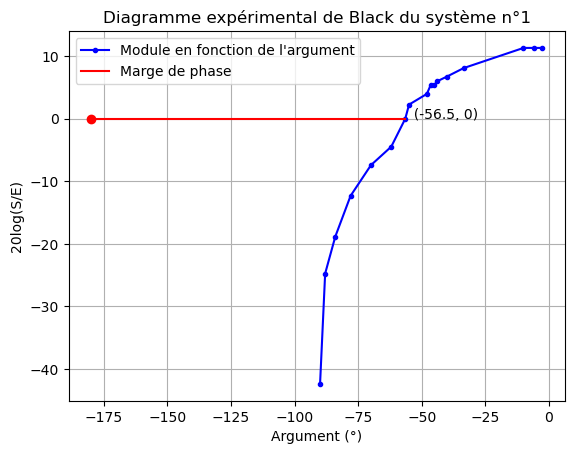
\includegraphics{Diagramme de Black experimental 2.1.png}
\end{center}

On remarque que ce diagramme a l'allure d'un passe-bas du $1^{er}$ ordre ($A > 0$, $\varphi \in [0^\circ,-90^\circ]$).
\\Graphiquement, la marge de phase (écart en phase entre le point à -180° et la courbe lorsque le gain est nul (sur l’axe des abscisses)) vaut $-56.5 - (-180) = 123.5^\circ$. Nous pouvions déjà déterminer la marge de phase sans le diagramme car nous avions déjà trouvé la fréquence pour laquelle $\frac{S}{E} = 1$.
\\Il suffit ensuite de mesurer le déphasage pour cette fréquence et d'y additionner 180.
\newpage


\begin{itemize}
    \item Système 2
\end{itemize}

\underline{Nature du système} : De même que pour le système 1, à fréquences très basse ($f \ approx 10$Hz), l'amplitude de la sortie est amplifiée, et pour des fréquences très élevées, l'amplitude de la sortie est quasiment nulle.
\\De plus, on remarque que pour $f = 5$Hz, le quotient de l'amplitude de la sortie (S) sur celle de l'entrée est supérieur ($\frac{S}{E} = 2.26$) que pour $f = 1$Hz ($\frac{S}{E} = 2$). On interpète ceci comme étant une résonance du système autour de la fréquence 5 Hertz.
Ainsi le système 2 est un passe-bas du $2^{\grave{e}  me}$ ordre. Pour déterminer la fréquence de coupure, nous savons qu'à cette fréquence, pour un filtre passe-bas du $2^{\grave{e}me}$ ordre, le déphasage vaut $-90^\circ$ ($A = 2 > 0$). Ainsi, on trouve $f_0 \approx 7.57$Hz donc $\omega_0 \approx 47.5$Hz.

Nous pouvons désormais mesurer les différents points nécessaires pour tracer le diagramme de
Black :
Comme nous avons déjà un ordre de grandeur de la pulsation de coupure, nous mesurons le module
et l’argument à des fréquences séparées par des intervalles plus petits lorsque ces fréquences sont
proches de $\omega_0$ et on agrandit les intervalles lorsqu’on s’en éloigne.
\begin{center}
    \begin{tabular}{ |p{3cm}|p{3cm}|p{3cm}|p{3cm}| }
        \hline
        \multicolumn{4}{|c|}{Points du diagramme de Black du système 2} \\
        \hline
        Fréquence $f$(Hz) & $\mid T \mid = \frac{S}{E}$ & $20 \log(\mid T \mid)$ & Déphasage $\varphi $ (°)\\
        \hline
        0.5 & 1.95 & 13.36 & -2.51 \\
        0.6 & 1.95 & 13.36 & -4.70 \\
        1.2 & 2 & 13.86 & -9.32 \\
        2 & 2.024 &  14.10 & -15.95 \\
        3 & 2.1 &  14.84 & -25.33 \\
        4 & 2.14 &  15.22 & -36.80   \\
        5 & 2.26 & 16.31 & -49.80 \\
        6 & 2.21 & 15.86 & -65.47 \\
        7 & 2.02 & 14.06 & -82.9\\
        \hl{$7.55 = f_0$} & 1.95 & 13.36 & -90\\
        8 & 1.83 &  12.09 & -97 \\
        10 & 1.30 &  5.25 & -118.5 \\
        11.5 & 1 & 0 &-130 \\
        15 & 0.57 & -11.24 & -145 \\
        25 & 0.24 & -28.54 & -161 \\
        35 & 0.14 & -39.32 & -166 \\
        50 & 0.07 & -53.19 & -170 \\
        100 & 0.023 & -75.45 & -175 \\
        \hline
        \end{tabular}
    \end{center}

    \newpage

    Voici le diagramme de Black expérimental : 
    \begin{center}
        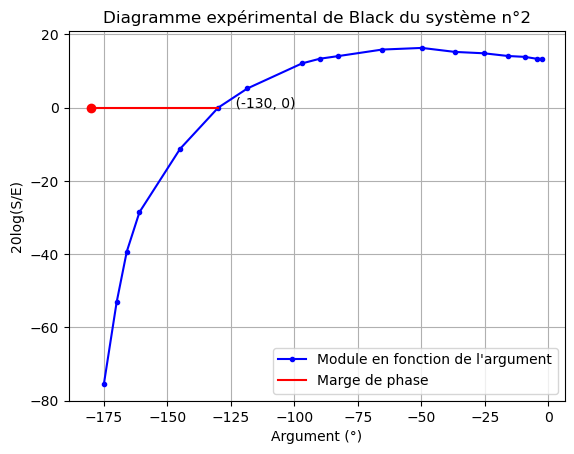
\includegraphics{Diagramme de Black experimental 2.1 Syst 2.png}
    \end{center}
    On remarque que ce diagramme a l'allure d'un passe-bas du $2^{\grave{e}me}$ ordre ($A > 0$, $\varphi \in [0^\circ,-180^\circ]$ et résonance).
    \\Graphiquement, la marge de phase vaut $-130 - (-180) = 50^\circ$.

    \section{\itshape Réponse indicielle.Réponse Harmonique.Identification}

    Le but de cette partie est dde modéliser notre système par une fonction de transfert. Pour cela, nous allons effectuer un essai indiciel ou harmonique sur les deux systèmes.
    \subsection{\itshape Travail Préparatoire}
\begin{itemize}
    

    \item  \underline{\itshape Caractéristique statique} : Pour un système linéaire la caractéristique statique est une
    droite passant par l'origine, dans une zone linéaire la pente de cette droite est
    l'amplification statique du système.

    \item \underline{\itshape Système du $1^{er}$ ordre} : Soit la fonction de transfert de $1^{er}$ ordre $F_1(p) = \frac{A}{1 + \tau p }$. Ici A représente le gain/l'amplification statique et $\tau$ représente la constante de temps (en secondes) du système.
    Pour représenter la réponse indicielle, nous savons que pour une entrée $e(t) = X_0\times\mathcal{U}(t)$, la réponse est de la forme $y(t) = AX_0(1-e^{\frac{-t}{\tau}})\mathcal{U}(t)$ avec $A$ et $\tau$ les éléments caractéristiques de $F_1(p)$.
    Ici, lessai indiciel est modélisé avec A = 2, $X_0 = 1$ et $\tau = 0.2$s
    \begin{center}
        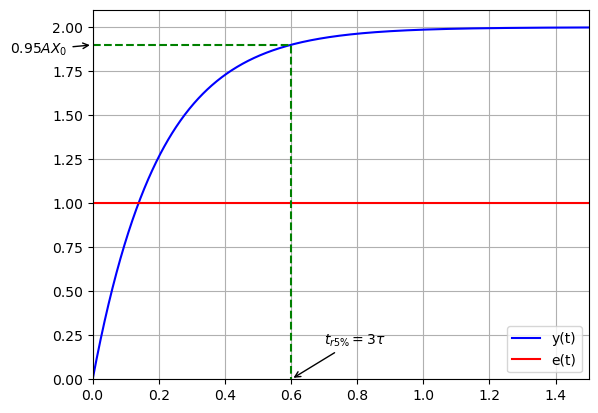
\includegraphics{Reponse_indicielle_prem_ordre.png}
    \end{center}


\end{itemize}
\end{document}